\documentclass[conference,10pt,letterpaper]{IEEEtran}
\usepackage{graphicx,booktabs,amsmath,amssymb,url}
\usepackage[hidelinks]{hyperref}
\graphicspath{{figures/}}
\newcommand{\system}{DataVine}
\newcommand{\aicredit}{\par\noindent{\footnotesize Drafting assistance: OpenAI Codex~\cite{codex}.}\par}
\input{results/numbers.tex}
\input{results/preloaded-numbers.tex}
\input{results/upgrade-numbers.tex}
\title{DataVine: Separating Task Dispatch, Data Readiness, and Execution Admission in Scientific Workflows}
\author{\IEEEauthorblockN{Anonymous submission draft}}
\begin{document}
\maketitle
\begin{abstract}
Scientific workflow runtimes must decide when a task is logically eligible,
where its inputs should be obtained, and when a worker should execute it.
Binding these decisions to a single admission event can leave computation
waiting for data coordination; advancing them independently can instead
create excessive staging and resource pressure. DataVine makes these three
decisions explicit. A logical scheduler dispatches eligible task descriptions,
a data controller owns intermediate identities and replica lifetimes, and
worker agents resolve inputs when execution opportunities approach. A bounded
worker queue is distinct from a feedback-controlled execution window. Physical
completion can release descendants before background backup, while requested
outputs have a separate durable-admission boundary. The implementation retains
individual task attempts and supports recall of queued, unstarted work.
Logical scheduling remains single-owner while Controller RPC handling and
durable-output persistence use independent data-plane concurrency pools.
We evaluate a complete ATLAS Open Data diphoton analysis, concurrency and
preparation controls and 2,048-task graphs across one
to eight distinct physical hosts. The analysis processes 36.56 million events
with exact agreement in all selection counts and histogram bins. Under matched
dependency preloading, DataVine elastic has a median paired completion-time
advantage of $\UpgradeAtlasElasticSpeedup{}\times$ over TaskVine. Fixed admission is
competitive with elastic admission; cold initialization and distributed
data-heavy chains expose substantial limitations. The artifact contains
\UpgradeTrials{} accepted trials in five randomized blocks per configuration
and \UpgradeRegressionPassed{} passing regression gates. The evidence supports
an explicit execution-boundary design, while limiting claims about adaptive
control and data-path scalability.\cite{codex}
\end{abstract}
\begin{IEEEkeywords}
scientific workflows, distributed runtime, intermediate data, admission control
\end{IEEEkeywords}

\section{Introduction}
Scientific applications increasingly execute as dependency graphs of short
computations and intermediate objects. The performance problem extends beyond
placing a runnable task on a free core: a successor must find its inputs, the
runtime must preserve those inputs for other consumers or recovery, and a
worker must distinguish work that is waiting from work that can use a CPU.
As tasks become shorter, repeated coordination at these boundaries can occupy
a substantial part of the interval between useful computations.

In a conventional design, the same single-threaded manager handles both
logical scheduling (dependency checks, dispatch, retries, and completion) and
data-lifecycle coordination. A large workflow amplifies the latter demand:
each intermediate input or output can trigger identity lookups, peer-copy or
checkpoint admission, stage-in or stage-out coordination, acknowledgements,
and garbage-collection updates. The bytes may move directly between workers,
but the manager still serializes much of the control and lifetime bookkeeping.
When these events arrive faster than one reactor can drain them, the manager
becomes the bottleneck and workers can remain idle even when runnable work
exists.

Existing systems already exploit local intermediate storage and peer transfer.
TaskVine manages an ensemble's storage and transfers~\cite{taskvine}; its use in
high-energy physics demonstrates the importance of both data and function
execution costs~\cite{hep}. Consequently, a credible next step cannot be to
rediscover local caching or replace one copy path with another. The question is
which component should own each decision, and which events must precede a
successor's execution.

Consider a task whose producer has finished on worker A. Worker B may have an
execution opportunity before a backup copy has reached persistent storage.
Waiting for backup before making the successor eligible needlessly orders
recovery work before computation in the failure-free case. Yet immediately
preparing every eligible successor can fill B's disk or memory with work that
will wait in its queue. Increasing concurrent processes can hide some waits,
but a fixed factor can also intensify competition during compute-heavy phases.
These are related ordering and admission problems.

Our central design choice is to expose three boundaries: logical dispatch,
physical input preparation, and execution admission. DataVine's scheduler owns
DAG eligibility and task attempts; its data controller owns named intermediates,
replicas, and retention; workers own the final preparation and execution gates.
A task description can wait cheaply on a worker before its input sandbox is
prepared. A bounded queue absorbs dispatch latency while a separate execution
window responds to current CPU, runnable-process, and memory pressure.
The design preserves explicit coordination at ownership transitions rather than
claiming that independent components never communicate.

The research contribution is the concrete interaction of these boundaries for
file-producing scientific tasks. Consumer-driven data lookup, separated storage
planes, and local scheduling queues all have precedents~\cite{hoplite,pocket,apollo}.
DataVine does not claim to introduce those primitives. Its hypothesis is that
allowing a logically eligible task to be assigned before local input readiness,
while postponing preparation until execution approaches, can reduce coordination
waiting without staging the full dispatch queue. An aggregate execution window
then provides a second control over work that actually consumes resources.

This paper makes three contributions. First, it specifies an ownership and
event-ordering model that separates task success, replica availability, execution
admission, and requested-output durability. Second, it implements that model
in an existing runtime, including generation-bound queued-task recall, deferred
preparation, and opt-in attempt tracing. Third, it provides matched experiments
that hold task bodies and scientific checks constant while varying preparation,
window policy, and runtime. These include a complete real-data diphoton analysis,
expanded function-slot controls, and five-block experiments
across distinct physical hosts. The results distinguish gains of the implemented
execution path from unsupported claims that feedback or extra concurrency
alone explains them.

The central scalability consequence is that serialized logical scheduling does
not also serialize data-plane service work. The manager remains the single
owner of logical DAG state and dispatch, while Controller RPC handling and
durable-output persistence use independent concurrency pools. We measure the
resulting manager/data-plane separation explicitly and report the shared-state
boundary where metadata scaling stops.

The scope is intentionally testable. Current routing is local-first, then a
live peer, with an admitted controller backup as fallback. It is not a learned
three-way optimizer over peer, controller, and shared filesystem. Likewise,
the controller is a distinct owner but is not demonstrated to scale without
bound; worker overcommit is a heuristic with measurable failure modes. We
report these limits alongside the measurements so that the architecture can
be assessed independently of broader, unsupported novelty claims.

\section{Background and Motivation}
\subsection{Four events that need not coincide}
For a producer $u$ and consumer $v$, distinguish producer success $S_u$,
consumer dispatch $D_v$, consumer input readiness $R_v$, and consumer execution
$E_v$. A valid execution requires the relevant inputs at $E_v$; it does not
inherently require those inputs to be present on the selected worker at $D_v$.
For an intermediate with asynchronous backup, denote backup admission by $B_u$.
A policy may permit $S_u \prec D_v$ and $R_v \prec E_v$ without imposing
$B_u \prec D_v$. This is an ordering permission, not a guarantee that a
particular transfer or backup finishes before another event.

Requested outputs introduce a different boundary. A user observing a final
result needs the service's promised durability, so physical task completion
alone cannot establish workflow-result availability. Separating these events
allows the runtime to move successors forward while retaining a stronger
condition at the user-visible result interface.

The bottleneck is observable before introducing a new scheduling policy.
Figure~\ref{fig:bottleneck-motivation}(a) increases one-MiB durable objects
from 64 to 1,024 at a fixed four-worker topology: service time grows from
0.87 to 13.64 seconds while manager owner work stays below 28 ms after
isolation. In (b), 4 GiB remote fan-in throughput falls from 542.8 to
442.9 MiB/s as endpoints grow from 16 to 64, with Controller CPU near
36--37 seconds. The matched 20,000-task comparison (c)--(d) sends 64.1 MiB
through the coupled manager and completes in 160.4 seconds, versus 0.04 MiB
and 10.0 seconds for the separated path (16.1$\times$ median). These results
motivate separating logical scheduling from data-lifecycle service.

\begin{figure*}[t]
\centering
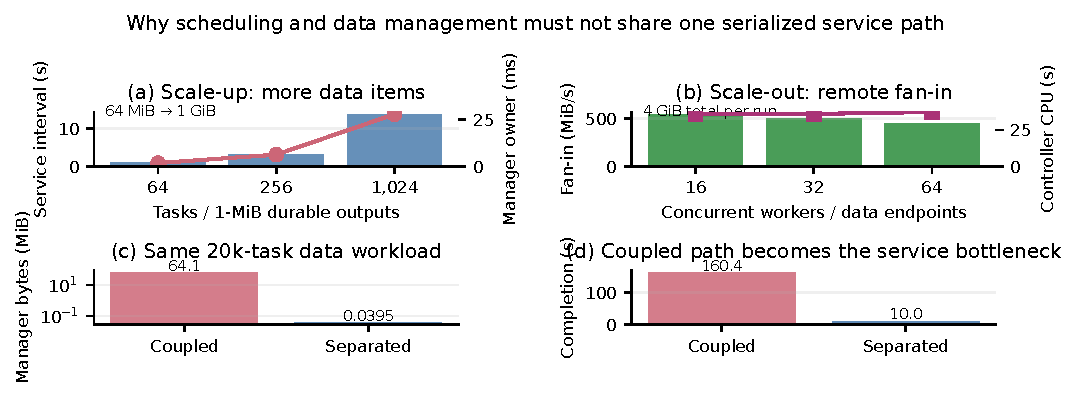
\includegraphics[width=.98\textwidth]{bottleneck-motivation.pdf}
\caption{Motivation evidence from real runs. (a) Fixed four-worker by two-core
scale-up with one-MiB durable outputs; the data-plane service interval grows
with objects while manager owner work stays small after separation. (b) Remote
Controller fan-in with 4 GiB total payload; adding endpoints exposes a shared
service boundary. (c)--(d) Matched 20,000-task data-intensive comparison: the
coupled path carries manager data-plane traffic and is slower, while the
separated path keeps payload service outside the scheduler. Bars use retained
medians; source hashes and raw runs are in the artifact.}
\label{fig:bottleneck-motivation}
\end{figure*}

\subsection{Queue depth is not executable capacity}
Let $Q$ be the maximum number of assigned function calls on a worker, and $W$
its current execution window. For $C$ allocated cores, a queue with $Q>C$
can buffer descriptors without requiring $Q$ executing processes or $Q$ fully
prepared input sandboxes. A conventional single limit obscures which form of
concurrency is increasing. DataVine makes $Q$ and $W$ distinct and uses the
availability of an execution opportunity to gate preparation.

A simple operational decomposition helps interpret measurements. A task's
observed worker residence includes waiting before preparation, preparation
itself, waiting after preparation, and execution. Increasing $Q$ primarily
changes what work is available locally; increasing $W$ changes competition
among executing or input-waiting calls. Neither necessarily reduces the
critical path. On a computation-bound phase, more processes may only increase
contention. On a data-waiting phase, a larger window may expose otherwise idle
CPU capacity. Measurements must therefore cover both regimes and transitions.

\subsection{What the motivating comparison must preserve}
A comparison against a baseline that sends every intermediate through a central
client would not isolate DataVine's control boundary. Our TaskVine baseline uses
its futures interface, temporary intermediate outputs, fork-based function
libraries, and the same kernel code. It benefits from the existing runtime's
peer-transfer and caching machinery. Every graph retains individual tasks;
there is no task fusion or replacing a chain with a single process.

Task grouping also advances some dependency knowledge toward workers~\cite{grouping}.
It must not be dismissed as fusion. Similarly, workflow-aware prefetch can
overlap movement and computation even if assignment requires prepared inputs.
The relevant distinction is the event at which assignment becomes legal, not
whether a system has asynchronous operations. Our eager/deferred ablation
isolates preparation timing within DataVine; it is not presented as a complete
reimplementation of either grouping or a prepared-node scheduler.

\section{Design}
\subsection{State ownership and interfaces}
Figure~\ref{fig:architecture} identifies the owners of the three decisions.
The workflow runtime accepts a graph of tasks and named data dependencies.
The scheduler maintains logical task states, unresolved dependency counts,
dispatch choices, and retry generations. It does not select a concrete source
replica for every task input during placement. The data controller maintains
DataID records, available replicas, invalidation, retention, and backup state.
Each worker agent maintains its local view of materialized data and performs
input resolution and movement. The generic TaskVine manager remains the sole
owner of the underlying task-manager API.

\begin{figure}[t]
\centering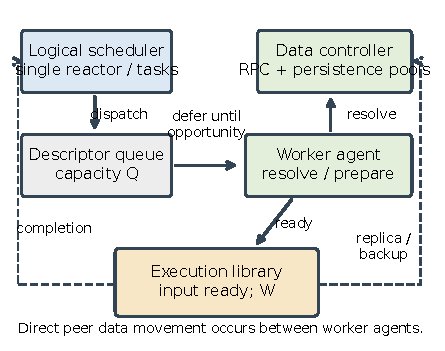
\includegraphics[width=\columnwidth]{architecture.pdf}
\caption{DataVine ownership and gates. Dashed arrows carry completion and
lifecycle information; data transfer does not route through the logical
scheduler. The manager and controller still perform coordination work.}
\label{fig:architecture}
\end{figure}

An input reference denotes data identity rather than a placement-time pathname
on a specific peer. The worker checks for a usable local copy, asks the
controller for a source when needed, and resolves that identity to a physical
input in the task sandbox. Replica location can change between dispatch and
preparation without changing the logical DAG edge. Conversely, a stale source
is not evidence that the producer's logical output should be accepted from a
different, obsolete attempt. Generations bind attempts and their control
messages to the scheduler's current state.

Separation does not remove all per-file work from the workflow runtime.
Completing a logical attempt still updates pending consumers and coordinates
mark-dead operations with the controller. The design changes ownership of
replica decisions, rather than asserting a zero-cost control path. This
qualification matters at high task rates, where serialized manager send,
status handling, and lifecycle operations can become dominant.

\subsection{Dispatch before local readiness}
After a producer's successful physical attempt is accepted, the scheduler
updates logical dependencies and makes newly eligible consumers dispatchable.
The scheduler may assign a consumer before its destination has prepared the
input. The assigned descriptor waits in a bounded worker queue. For the
fork-based DataVine execution path, the worker first checks whether a suitable
execution-library opportunity exists; absent one, it postpones the agent's
preparation operation. Once preparation starts, the agent resolves generated
inputs and initiates required transfers. Execution remains conditional on
input readiness, library availability, and resource matching.

This order prevents a deep descriptor queue from automatically becoming an
equally deep collection of staged sandboxes. It also changes prefetch distance:
earlier preparation can hide a long transfer, whereas later preparation can
reduce unnecessary staging. The correct empirical question is where this
tradeoff changes sign. We therefore implement an eager preparation control
that bypasses only the preliminary execution-opportunity check. It retains
all input-readiness and actual execution checks. The control is not an unsafe
mode that executes without data.

The design does not provide two independently optimized transfer and compute
windows. Preparation and execution remain related through the library gate;
input transfer may occupy an opportunity that could otherwise serve another
call. Decoupling those windows further is a possible extension, but requires
separate bounds on transfer bytes, sender contention, and prepared-data
occupancy. We avoid attributing such a mechanism to this implementation.

\subsection{Data path and retention}
For each generated input, a worker uses a valid local replica when available.
Otherwise the controller resolves a live source; peer data can be transferred
directly between workers. A controller backup is eligible as fallback only
after its admission has completed. This ordering avoids publishing an
incomplete backup as if it were a usable replica. A peer becoming unavailable
can trigger a new resolution rather than forcing the scheduler to encode a
permanent source into the task descriptor.

The default intermediate policy retains live worker copies and performs
controller backup in the background. Controlled performance comparisons can
select worker-local intermediates, disabling this backup while preserving
requested-output handling. These configurations have different recovery
costs and must not be combined into a single speedup claim. Shared-filesystem
experiments in the wider artifact explore a possible alternative data path;
the production worker does not currently choose it through an adaptive
three-way cost model.

Data lifetime is tied to consumers and requested outputs, not merely to the
producer's return. Once the graph can establish that an intermediate is no
longer needed, lifecycle updates permit reclamation. Dynamic graph extension
makes this more subtle: an open workflow can introduce a future consumer, so
retained data may accumulate until sealing establishes a closed consumer set.
A bounded descriptor queue is therefore not a global bound on intermediate
storage. The controller's retention policy and workflow closure remain part
of the capacity model.

\subsection{Worker execution feedback}
The default dispatch capacity is $Q=8C$. The elastic execution window starts
at $W=2C$ and samples worker pressure every 250\,ms. CPU saturation, runnable
pressure, and memory are separate signals. In the current policy, CPU at or
above 95\% together with runnable pressure above $3C$ for two samples reduces
the window by $C$, with a floor of $2C$. The $3C$ value is a feedback threshold,
not a hard bound on concurrent processes. Memory pressure at 80\% causes a
stronger backoff and drain; declared task memory supplies an additional
admission check.

When calls are waiting, low measured CPU (below 85\%) and memory (below
70\%) allow multiplicative growth; otherwise an eligible growth step adds
$C$, capped by configured library slots. The policy holds near its 90\% CPU
target when the runnable population is at least $C$, and inserts a cooldown
after backoff. Before increasing $W$, it estimates a memory-limited window
from the current running count $R$ and measured memory fraction $m$:
\begin{equation}
W_{\mathrm{next}}\leftarrow\min\left(W_{\mathrm{candidate}},
\max\left(R,\left\lfloor0.8R/m\right\rfloor\right)\right).
\end{equation}
This guard applies when $R>0$ and $m>0$. A memory-fraction increase above
0.10 in one sample defers growth to avoid extrapolating from a partially
faulted-in footprint. These thresholds are implementation choices tested
against fixed windows, not tuned optima. Shrinking admission does not kill
running calls: the population drains before newly permitted calls enter.

The policy aims to respond to current aggregate behavior without requiring
accurate runtime predictions for every task class. It is not a proof of memory
safety or stability. A task can allocate more memory than declared between
samples, and low CPU usage does not imply that more processes will help a
memory-bandwidth-bound workload. Fixed windows at $C$, $2C$, and $4C$ therefore
remain essential controls. We report the best tested fixed choice as an
empirical reference, not as an oracle for every possible setting.

\subsection{Recall, failure, and result visibility}
An assigned task that has not begun execution may be recalled under its
current generation. The runtime distinguishes that state from a running
attempt; recall is not process migration. Retrying under a new generation
must prevent delayed messages from an earlier attempt from advancing the
new attempt's state. This is especially important when worker loss,
re-resolution, and completion notification overlap.

Physical success releases logical descendants before background persistence,
but user-visible requested results wait for durable admission. A completed
worker task and a completed workflow result are thus deliberately different
states. Recovery tests exercise worker loss, lifecycle handling, and replay.
The contract does not give arbitrary user side effects exactly-once semantics.
A retried task that writes to an external database needs application-level
idempotence or a stronger transactional interface.

Finally, controller-local storage determines the failure domain. A backup on
the controller's local temporary filesystem survives a worker's loss but is
not a cross-host durable service if that controller host disappears. We make
this assumption explicit rather than generalizing worker-loss tests into a
claim of controller-host fault tolerance.

\section{Implementation}
\subsection{Runtime integration}
DataVine is implemented within the TaskVine codebase using a C workflow
runtime, scheduler, controller protocol, and worker agent, with a Python
workflow interface. One workflow process owns a reactor and the sole manager
API owner. Static graph submission declares task and edge bounds; dynamic
extension retains the same data-identity and attempt contracts. Python
functions use a fork-based execution library. Each logical node generates an
individual physical attempt in the failure-free experiments; retries remain
visible rather than being hidden as task fusion.

The baseline service demand is therefore mixed: one manager reactor drains
dependency and dispatch events while also receiving the data-lifecycle events
caused by intermediate objects. Replica or checkpoint decisions, stage-in and
stage-out acknowledgements, and object-retention or garbage-collection updates
all consume that serialized control path, even when the payload itself is
transferred peer-to-peer. The cost grows with the number of data items and
their consumers, so a worker-side compute shortage is not required for the
manager to saturate.

The service keeps the workflow manager's reactor as the serialized owner of
logical scheduling, while the data-plane endpoint has independent RPC event
threads and Controller persistence workers. RPC threads process authenticated
agent metadata and object requests; persistence workers perform the queued
stream, fsync, verification, and commit path. The default service uses one RPC
thread and 16 persistence workers. The separation is configurable for the
scaling validation, but shared metadata state still imposes a measured limit.

The implementation uses explicit generated-input descriptors and data IDs.
The worker agent handles local materialization and source resolution; the
logical scheduler need not insert a concrete peer endpoint into every task
at placement time. Controller requests are authenticated, and the wire
contracts are versioned. Small callable payloads may be inlined within the
existing size bound, while larger payloads use the corresponding source path.
These encoding optimizations reduce some setup work but are not themselves
the contribution evaluated here.

\subsection{Preparation ablation and observability}
We added a worker environment control selecting deferred or eager preparation.
Deferred is the unchanged default. Eager skips only the check that postpones
agent preparation when an execution-library opportunity is absent. An invalid
setting produces a notice and retains the deferred behavior. The setting is
read once per worker process, making each experimental condition explicit and
stable throughout a trial.

Optional attempt tracing records worker receipt, first preparation start,
preparation readiness, execution start, and completion. Collection is disabled
by default and applies only to auxiliary-payload tasks. The additional process
fields are generic timestamps; DataVine-specific selection and logging remain
in the worker integration point. This preserves the repository's module
boundary checks. Each trace is local to one worker clock. We compute local
intervals and never subtract timestamps from different hosts to infer latency.

For a completed attempt with timestamps $t_r,t_p,t_d,t_e,t_f$, the validation
checks $0<t_r\leq t_p\leq t_d\leq t_e\leq t_f$. The intervals $t_p-t_r$,
$t_d-t_p$, $t_e-t_d$, and $t_f-t_e$ distinguish queue waiting, preparation,
post-preparation waiting, and execution. A missing trace is not interpreted as
zero waiting. Instrumented functional runs verify one trace per physical
attempt; uninstrumented campaigns provide the primary performance samples.

\subsection{A stronger concurrency baseline}
Stock TaskVine fork libraries reject configurations with more function slots
than library cores. The one-slot-per-core baseline retains that behavior.
To test whether a speedup can be explained merely by a larger fixed window,
we also construct an experimental TaskVine control with two or four slots per
allocated core. This control changes only the startup restriction in a private,
generated library file. It does not alter repository Poncho sources, advertise
extra physical CPUs, or increase the worker's actual allocation. The worker's
slot accounting still determines admitted function calls; native math libraries
are limited to one thread.

We label these configurations as extended TaskVine throughout the evaluation.
They are not claimed to be supported stock configurations or a reimplementation
of DataVine's feedback. Their purpose is to challenge attribution: DataVine
should be compared against a baseline capable of exposing more concurrency,
not just against an artificially restrictive one. The generated source hash
and the exact transformation are retained with the trial evidence.

\subsection{Controlled dependency initialization}
A generated DataVine executor prototype preloads an explicit module list before
its readiness handshake. It is selected through the existing executor-path
configuration and leaves the default executable intact. The artifact records
the base executable hash, generated hash, and imported modules. The matching
TaskVine library hoists exactly those modules. Preloading is a deployment
control, not a new scheduling algorithm or a claim that arbitrary initialized
libraries can safely be inherited across fork. Native numerical libraries are
limited to one thread in the measured configuration.

\subsection{Recall destination progress}
The initial remote experiments exposed a liveness defect in dense least-loaded
dispatch. A successfully recalled task retained a reserved destination, while
reoffering other lower-load workers allowed the same incompatible worker to be
selected repeatedly within a bounded pass. A ready task could consequently
remain unassigned after all other work drained. The diagnostic trace showed
one such task still READY with idle execution libraries.

The fix preserves both destination binding and least-loaded preference. At the
start of each pass, the worker pool compacts stale generation entries and clears
visit marks. Selection considers each live offered worker at most once during
that pass. Reoffering an incompatible worker preserves future availability but
does not hide another worker in the current pass. This adds no per-task worker
list allocation. A deterministic regression covers repeated offers, unequal
loads, and recycled worker slots. The original four-worker diagnostic timed
out before the fix and completed with all results validated after the fix.
Pre-fix campaign data is retained separately and excluded from the primary
performance figures.

\subsection{Correctness and compatibility checks}
The full DataVine regression suite passes \UpgradeRegressionPassed{} gates. Focused
runtime acceptance executes the same 32-task phase graph under eager and
deferred preparation, verifies every logical result and physical attempt
count, and checks all trace orderings. The existing generic TaskVine serverless
test also passes in a private scratch directory; it covers both direct and
fork function libraries and validates returned values and file output. These
checks establish exercised compatibility, not exhaustive correctness for all
interleavings. The failure-injection experiment complements them by removing
only worker jobs owned by its own factory.

\section{Evaluation}
\subsection{Questions and experimental contract}
We ask whether the separated boundaries help a complete scientific analysis,
whether fixed concurrency or dependency initialization explains the gain,
and how the result changes across physical hosts. The primary evidence comprises
\UpgradeTrials{} accepted trials in five randomized blocks per configuration.
Figures show medians and observed ranges. With five samples we report paired
ratios and wins, not precise population confidence intervals.

Colocated controls use two four-core workers with disjoint affinity within an
eight-CPU allocation. Application studies use their own
allocation. The control continuation retains complete comparison blocks and
reruns an interrupted block in full; it never pairs runtimes from different
allocations. Physical-host scaling holds eight persistent batch allocations
on eight distinct hosts of the same machine class and selects nested subsets
of one, two, four, and eight hosts, with eight CPUs per worker. All task records
must match an admitted worker's declared CPU set. These are CPU shares with
explicit affinity, not exclusive whole-node reservations. Other users and
submission-host load can still introduce contention.

Each trial starts a fresh service or manager, admits its complete pool, then
times graph construction, submission, execution, every sink fetch, and local
sink fsync. DataVine also admits requested outputs durably at its controller;
the persistence operation count is consequently not identical. Worker-local
intermediates are used in both backends. Pool admission is excluded and
recorded separately. Libraries have no additional readiness barrier, so
residual library startup remains inside the interval.
The TaskVine baseline uses the ordinary FuturesExecutor and temporary-output
path in the same checkout, including its shared function-credit implementation;
it is not a separately built, unmodified upstream release.

Python is 3.10 with NumPy 1.26.4; the analysis additionally uses Uproot 5.6.8,
Awkward 2.8.7, and Vector 1.6.3. Dependencies are copied to node-local storage
before colocated campaigns. Both libraries explicitly preload the same
modules before forking, except in the labeled cold controls. DataVine's
generated executor exists before service startup, and its hash must match
the executable actually received by every worker. This check caught and
excluded an earlier harness version that silently deployed the default
executor. Failed, interrupted, and incompatible trials remain diagnostic
artifacts; none contributes a zero bar or a replacement success.

\subsection{Serialized scheduling and concurrent data-plane work}
The first architectural claim is that data-lifecycle service demand need not
consume the manager's scheduling reactor. In the conventional single-reactor
path, dependency scheduling and dispatch share that reactor with replica or
checkpoint coordination, stage-in/out acknowledgements, and retention or
garbage-collection updates. The workflow process retains one owner for
logical scheduling and TaskVine manager state, but the service endpoint handles
data-plane RPC connections with an independent event-thread pool, while
requested-output persistence runs in a separate Controller data-worker pool.
The current-build validation exposes both counts as
\texttt{DATAVINE\_RPC\_THREADS} and \texttt{DATAVINE\_DATA\_THREADS}; defaults
remain one RPC thread and 16 data workers. The manager never becomes the path
for the durable output bytes, although it still receives the corresponding
completion and lifecycle notifications.

Table~\ref{tab:controller-decoupling} holds the single-thread scheduling
service and workload fixed while changing only the Controller data-worker
count. Two repetitions at each point produced 26.9, 43.9, and 63.7 tasks/s
medians for one, four, and 16 data workers, respectively, a 2.37$\times$
median improvement from one to 16. Every run completed 256 one-MiB outputs
and verified all 268 MiB of durable bytes. The manager's owner-execute time
was 6.9--27.6 ms across these runs, while the end-to-end service interval was
3.1--14.6 s. This separates the manager's scheduling control path from the
measured durability work, while exposing local-filesystem variability. The
experiment does not claim that all data operations scale linearly; it tests
whether data-plane work that would otherwise share the manager's serialized
service path can be served concurrently.

\input{results/controller-decoupling-table.tex}

The worker-local control completes the same 256 tasks at 461.7 and 453.1
tasks/s with one and 16 data workers, respectively, and creates no durable
Controller files. Manager owner-execute time remains 1.59 and 1.58 ms. Thus
the thread-sensitive cost is in requested-output data management, while the
logical scheduling path remains stable.

An unbatched metadata-RPC control processed 39.5k publish and 37.8k resolve
records/s with one client connection. Sixteen concurrent connections reached
91.5k and 84.6k records/s even with one RPC event thread; 16 event threads
reached 98.9k publish records/s. The small incremental gain and the resolve
plateau are expected: metadata still uses shared controller state. The result
supports independent data-plane concurrency and identifies its remaining
serialization boundary; it does not claim unlimited Controller scaling.
The complete protocol regression with 16 RPC and 16 data threads passed
submission, restart, compare-and-swap append, journal recovery, corruption
rejection, the 1024-connection cap, and object-store deduplication.
The raw summary and source fingerprints are retained with the artifact.

\subsection{Complete ATLAS Open Data analysis}
We port the existing diphoton analysis accompanying ATLAS Open Data educational
materials~\cite{atlas-open-data}. The complete available sample contains 16
ROOT files, 9,861,498,743 bytes, and 36,564,144 collision events. The DAG has
374 read/decompression tasks, 374 photon-selection tasks, and 54 reduction
tasks: 802 individual attempts. Reads cover at most 100,000 events each;
selection consumes the actual jagged arrays, and an eight-way reduction
combines selection counts and the diphoton-mass histogram. There are no
synthetic sleeps or substituted numerical kernels in this application.

An independent run of the existing full-file analysis pins every input hash,
all seven selection counts, and all 60 histogram bins. Every accepted runtime
run agrees exactly, including 553,456 selected events. We preserve the reference
selection, including its permissive eta OR predicate; the purpose is runtime
equivalence, not a revised physics selection. A diagnostic implementation that
rearranged float32 mass arithmetic changed five selected events and was rejected.
The accepted version preserves the reference Vector operation order.
Exact numerical acceptance is platform-specific: a TaskVine replay on a second
platform selected 553,458 events against the primary reference's 553,456.
The unchanged independent reference on that platform reproduced every observed cut
and bin difference. We retain the rejected run, provide independently generated
platform-specific manifests, and do not assume cross-platform bitwise identity.
The primary performance figures continue to use the original allocation.

The complete ROOT dataset is copied and hashed once before the application
campaign. That setup cost is retained but excluded from workflow time. Reading,
decompression, selection, array serialization, intermediate delivery, reduction,
and durable sink admission remain inside the timer. OS caches are not flushed.
This is a complete educational analysis over real data on one compute host;
it is not a production collaboration analysis or distributed input-store study.

\begin{figure}[t]
\centering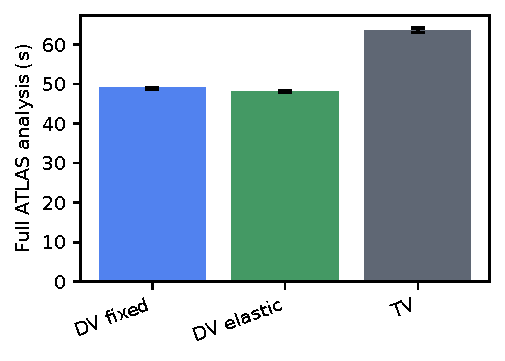
\includegraphics[width=\columnwidth]{upgrade-application.pdf}
\caption{The full 36.56-million-event ATLAS analysis. Five paired blocks,
802 individual tasks per run, and exact agreement with the independent oracle.
Bars are medians; whiskers are observed ranges.}
\label{fig:application}
\end{figure}
DataVine fixed and elastic complete in median \UpgradeAtlasFixedMedian{} and
\UpgradeAtlasElasticMedian{} seconds, versus \UpgradeAtlasTVMedian{} seconds
for TaskVine. Median paired completion-time ratios are
\UpgradeAtlasFixedSpeedup{} and \UpgradeAtlasElasticSpeedup{}, respectively.
The close fixed/elastic result is evidence against attributing this application
gain primarily to feedback. The comparison supports the implemented execution
path under the stated initialization and storage contract.

\subsection{Matched concurrency and preparation controls}
CPU chains contain 64 independent lanes of eight 50-ms process-CPU tasks,
with 1-KiB outputs. Hash chains use the same 512-task graph with 1-MiB outputs;
each consumer checks its parents' payload hashes. The phase DAG contains 256
tasks alternating 100-ms CPU work and actual node-local writes, fsync, and
reads with 256-KiB payloads and fan-in. Task bodies, graph structure, logical
result visibility, and sink acceptance are identical across backends.

\begin{figure*}[t]
\centering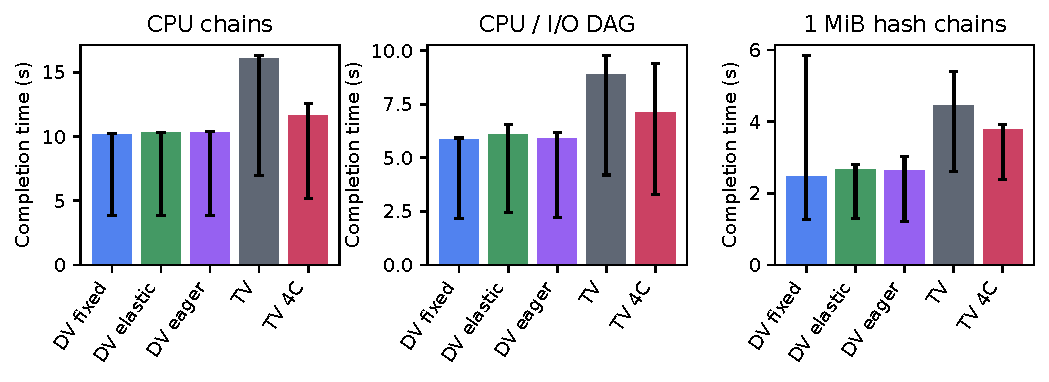
\includegraphics[width=.96\textwidth]{upgrade-controls.pdf}
\caption{Concurrency and preparation controls, five paired blocks each.
DV fixed uses one execution slot per core; DV elastic adapts its window;
DV eager also advances preparation. TV 4C is the explicitly extended fork
library with four slots per allocated core, not four times the CPU allocation.}
\label{fig:controls}
\end{figure*}
\begin{table}[t]
\centering\small
\caption{Median completion time in seconds for the matched controls.}
\input{results/upgrade-controls-table.tex}
\end{table}
The extended TaskVine control removes only the generated fork-library startup
guard against slots exceeding cores. Its physical allocation remains fixed.
It challenges the explanation that extra concurrency alone is sufficient.
Within DataVine, fixed, elastic, and eager controls are close on these graphs;
there is no consistent case here for making the adaptive window the principal
research contribution. End-to-end differences also include serialization,
graph submission, and result processing. They are not a factorial isolation
of scheduler and data-controller costs.

\subsection{Scaling across distinct physical hosts}
\begin{figure*}[t]
\centering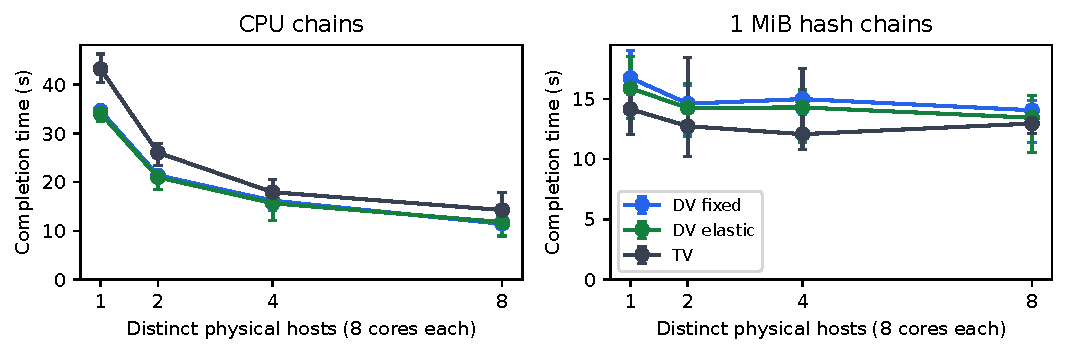
\includegraphics[width=.96\textwidth]{upgrade-scaling.pdf}
\caption{Fixed-size 2,048-task graphs on nested subsets of eight persistent,
distinct physical hosts, eight CPU shares per host. Five paired blocks;
medians and ranges. Nodes are not exclusively reserved.}
\label{fig:scaling}
\end{figure*}
The scaling graph has 256 lanes and eight stages. CPU tasks consume 100 ms
each and emit 1 KiB; the data case generates and hashes 1 MiB per task with
minimal additional CPU work. Separating these cases avoids interpreting a
CPU scaling result as a data-path scaling result. The same persistent pool
is used throughout; a continuation retains all completed non-grouping trials
and resumes the original randomized order after incompatible grouping trials
are removed from the comparison.

\input{results/upgrade-scaling-summary.tex}
The data-path result is particularly consequential: more remote endpoints can
add scheduling and delivery work without shortening the critical path. These
measurements bound the useful envelope of this implementation. They do not
establish controller capacity at 16 or more nodes, nor isolate whether manager
serialization, placement, or data-controller service dominates every plateau.

\subsection{Initialization, instrumentation, and CPU accounting}
The attribution campaign holds a single allocation and executes five paired
blocks at 1-KiB and 1-MiB payload sizes. It compares preloaded and cold libraries,
and instrumented and uninstrumented execution, independently for each backend.
This avoids inferring a cold-start effect from two different hardware campaigns.

\input{results/upgrade-attribution-summary.tex}
The cold controls retain DataVine's startup disadvantage rather than treating
preloading as a free default. Users must provision an explicit, fork-compatible
dependency environment. The prototype's executable override is now fail-closed:
an explicitly missing or non-executable path cannot silently select a different
executor. Performance evidence remains attached to its exact measured binaries;
the subsequent compatibility repairs have separate regression evidence.

Worker-lifetime CPU accounting includes worker and library startup and shutdown.
Task-body CPU excludes deserialization and some import costs. Optional process
sampling is non-atomic, and summed RSS can count shared pages repeatedly.
\begin{table}[t]
\centering\small
\caption{Median CPU seconds. DV uses fixed admission. Worker lifetime aggregates
both worker process trees; it excludes manager, controller, and client CPU.}
\input{results/upgrade-cpu-table.tex}
\end{table}
Similar task-body CPU and different worker-lifetime CPU support an explanation
involving runtime and library overhead, rather than cheaper numerical work.
They do not establish total cluster CPU savings: some work can move to the
controller, and the two timer scopes must not be subtracted as a full accounting.
The artifact separately reports these scopes and manager send/status timers.
Manager file-byte counters exclude peer traffic; we do not label them total
network bytes. Validation of 5,120 local-clock traces confirms one ordered
trace per instrumented physical attempt. Reconstructed stage occupancy counts
describe tasks in each stage, not physical prepared-data bytes.

\subsection{Correctness, failure injection, and remaining scope}
The retained measured build passes \UpgradeRegressionPassed{} DataVine regression
gates. The current configurable service build additionally passes the native
workflow protocol regression with both one and 16 RPC event threads and one and
16 Controller data workers.
Explicit invalid-executor tests require failure before service contact.
The runner verifies the loaded Python extension and records binary hashes,
preventing an installed older extension from masquerading as this build.

The retained recovery experiment removes three owned worker jobs from a
1,024-task workflow and validates all identities and 16 sinks after 18
resubmissions. Focused eager/deferred runs validate 32 ordered attempts per
mode, and generic serverless execution remains covered. These are exercised
semantics, not exhaustive failure coverage. Whole-node 16+ scaling,
prepared-node assignment, and exact sender-level traffic and prepared-byte
accounting remain open. Requested-output fsync is not controller-host-loss
durability, and no arbitrary external-side-effect exactly-once claim is made.

\section{Discussion and Limitations}
\subsection{When separation helps, and when it does not}
The proposed boundary is most promising when data coordination or input waits
are large enough to leave useful execution opportunities unfilled, but task
descriptors are cheap enough to queue. It can be less effective for long,
purely computational tasks; for short graphs dominated by startup; or for
workloads whose intermediates overwhelm available storage. A larger window
cannot manufacture bandwidth once senders, memory channels, or disks saturate.
An eager preparation policy may outperform deferred preparation when prefetch
latency matters more than prepared-data occupancy.

The logical scheduler currently uses a least-loaded choice rather than a
comprehensive locality cost model. Moving replica choice out of placement
simplifies one boundary but may incur more remote reads. Integrating locality
hints would require stating whether they are advisory, how stale hints are
handled, and whether they reintroduce synchronous source coordination. The
present architecture permits that extension; the present measurements do not
prove that it is unnecessary.

\subsection{Recovery costs and storage limits}
Worker-local intermediates expose a different recovery tradeoff from
background backup. Requested-output durability does not automatically protect
all intermediate state. Likewise, fsync on a controller-local filesystem
provides a host-specific contract, not replicated durability across host loss.
A future controller replication design would need explicit authority transfer,
log ordering, and failure fencing. Adding a second controller process without
those rules would not establish the stronger guarantee.

Open workflows can retain data for consumers not yet declared. Storage
credits, spill policies, and cancellation cleanup therefore deserve separate
capacity experiments. Memory sampling and declared-memory admission do not
bound every user allocation, and the current feedback ignores some bottlenecks.
An extension using transfer-byte credits or independent compute and transfer
windows should be evaluated against the current simpler policy, including
cases where extra state and control work make it slower.

\subsection{What the new evidence establishes}
The complete ATLAS analysis closes the gap between isolated numerical kernels
and an end-to-end workflow over real scientific data. It does not establish
production collaboration readiness, heterogeneous deployment, or distributed
dataset ingestion. The fixed/elastic comparison also changes the interpretation:
the execution boundaries and their ownership are the evaluated design, while
feedback remains an implementation choice whose incremental benefit is limited
on the tested graphs.

Five-block measurements across eight distinct physical hosts provide a larger
and more controlled scaling study than counting opportunistically colocated
workers. They still lack exclusive nodes, 16+ hosts, and a controller-capacity
sweep at fixed application work. The data-heavy results caution against assuming
that independent data ownership removes every centralized or placement cost.
Cold-library sensitivity similarly makes dependency preparation part of the
deployment contract, not an incidental detail that can be omitted from a claim.

Native grouping is now exercised with compatible start-credit semantics and
expanded windows. A prepared-node assignment policy remains an unimplemented
baseline; eager preparation alone is narrower than that policy. Exact sender
traffic and physical prepared-byte accounting remain necessary for stronger
claims about network or storage savings. Worker-lifetime CPU and ordered local
traces strengthen attribution but do not replace those measurements.
Together, these results support explicit ownership of logical scheduling and
data-lifecycle service as the paper's architectural contribution.

\section{Related Work}
\textbf{Data-aware scientific runtimes.}
TaskVine already manages in-cluster data and peer movement~\cite{taskvine}, and
its high-energy physics application combines data placement and function
execution improvements~\cite{hep}. DataVine builds on this runtime but moves
replica resolution and preparation timing across explicit owners. Task grouping
and WOW provide relevant locality and prepared-node alternatives~\cite{grouping,wow};
their boundaries differ from dispatching before local readiness.

\textbf{Separated data and recovery services.}
Hoplite and Pocket establish consumer-driven lookup and independent storage
services~\cite{hoplite,pocket}; ExoFlow separates execution from recovery under
a stronger exactly-once contract~\cite{exoflow}. DataVine does not claim those
primitives. The contribution under study is their interaction with
input-preparation timing, logical progress, and worker admission for
file-producing scientific tasks.

\textbf{Local queues and resource adaptation.}
Apollo and Sparrow study local queues, scheduling correction, and late binding~
\cite{apollo,sparrow}; adaptive allocation predicts resource needs from
observed tasks~\cite{adaptive}. DataVine binds descriptors early but postpones
physical preparation. Wasabi and Svalinn constrain claims about resource-aware
queuing, overbooking, and overload admission~\cite{wasabi,svalinn}. We do not
claim queuing, recall, overcommit, or CPU/memory feedback as individually novel.

\bibliographystyle{IEEEtran}
\bibliography{references}
\section*{Acknowledgments}
OpenAI Codex~\cite{codex} assisted with research synthesis, implementation,
experiment scripts, and drafting throughout this manuscript. The paper remains
an evidence-backed research draft requiring author review before submission.
\end{document}
